\documentclass[10pt,twocolumn,letterpaper]{article}
% PACKAGES ===================================================================================
\usepackage{iccv}
\usepackage{times}
\usepackage{epsfig}
\usepackage{graphicx}
\usepackage{amsmath,amssymb}
\usepackage{algorithm,algpseudocode}
\usepackage{subfig}

% Include other packages here, before hyperref.

% If you comment hyperref and then uncomment it, you should delete
% egpaper.aux before re-running latex.  (Or just hit 'q' on the first latex
% run, let it finish, and you should be clear).
\usepackage[pagebackref=true,breaklinks=true,letterpaper=true,colorlinks,bookmarks=false]{hyperref}

% ============================================================================================
% COMMENTS
% ============================================================================================
\newcommand{\stavros}[1]{{\textcolor{red}{[\emph{stavros}: #1]}}}

% ============================================================================================
% GENERAL DEFINITIONS
% ============================================================================================
\usepackage{xspace}
\def\sota{state-of-the-art}
\def\groundtruth{ground truth}
\def\CUB{CUB-200-2011}
\def\eg{\emph{e.g}\onedot} \def\Eg{\emph{E.g}\onedot}
\def\ie{\emph{i.e}\onedot} \def\Ie{\emph{I.e}\onedot}
\def\cf{\emph{c.f}\onedot} \def\Cf{\emph{C.f}\onedot}
\def\etc{\emph{etc}\onedot} \def\vs{\emph{vs}\onedot}
\def\wrt{w.r.t\onedot} \def\dof{d.o.f\onedot}
\def\etal{\emph{et al}\onedot}
\def\kmeans{\emph{k}-means}
\def\cpp{C\texttt{++}}
\def\matlab{MATLAB}
\def\matconvnet{MatConvNet}

% Chapters, Sections, Figures, Equations
\newcommand{\refchap}[1]{Chapter~\ref{#1}}
\newcommand{\refsec}[1]{Section~\ref{#1}}
\newcommand{\reffig}[1]{Figure~\ref{#1}}
\newcommand{\refeq}[1]{Equation~\ref{#1}}
\newcommand{\reftab}[1]{Table~\ref{#1}}
\newcommand{\refapp}[1]{Appendix~\ref{#1}}

% ============================================================================================
% MATH DEFINITIONS 
% ============================================================================================
\newcommand{\pd}[2]{\frac{\partial #1}{\partial #2}}
\newcommand{\mat}[1]{\mathbf{#1}} 
\renewcommand{\vec}[1]{\mathbf{#1}}
\newcommand{\set}[1]{\mathcal{#1}}
\newcommand{\inprod}[1]{{\left< \, #1 \, \right>}}
\newcommand{\R}{\mathbb{R}}
\def\abs{\operatorname{abs}}
\DeclareMathOperator*{\argmin}{argmin}
\DeclareMathOperator*{\argmax}{argmax}
\newcommand{\p}[1]{\vec{p}_{#1}} 	 % point with subscript
\newcommand{\norm}[1]{\left \lVert #1 \right \rVert} % norm


% \iccvfinalcopy % *** Uncomment this line for the final submission

\def\iccvPaperID{****} % *** Enter the ICCV Paper ID here
\def\httilde{\mbox{\tt\raisebox{-.5ex}{\symbol{126}}}}

\begin{document}
\title{AMAT: Computing the Medial Axis Tranform for Natural Images Using a Weighted Geometric Set Cover Approach}
\maketitle
%\thispagestyle{empty}


%%%%%%%%% ABSTRACT
\begin{abstract}
The medial axis transform (MAT) is a powerful shape abstraction that has been successfully
used in shape editing, matching and retrieval. 
Despite the MAT's long history, the lack of a definition and an evaluation criterion 
that accommodate color and texture have prevented its widespread use in tasks involving natural images.
In this paper we introduce Appearance-MAT (AMAT), by framing the MAT 
of natural images as a weighted geometric set cover problem.
We make the following contributions: 
i) we extend previous medial point detection methods for color images,
by associating each medial point with a local scale; 
ii) inspired by the invertibility property of the binary MAT, we also associate each medial point with a local encoding
that allows us to invert the AMAT, reconstructing the input image; 
iii) we describe a clustering scheme that takes advantage of the additional scale and appearance information 
to group individual points into medial branches, providing a shape decomposition of the underlying image regions.
In our experiments, we show \sota\ performance in medial point detection on
Berkeley Medial AXes (BMAX500), a new dataset of medial axes based on the established BSDS500 database.
We also measure the quality of reconstructed images from the same dataset,
obtained by inverting their computed AMAT.
Our approach delivers significantly better reconstruction quality \wrt to two baselines,
using just 10\% of the image pixels. 
Our code and annotations will be made publicly available.
\end{abstract}


%%%%%%%%% BODY TEXT %%%%%%%%%%%%%%%%%%%%%%%%%%%%%%%%%%
% ====================================================================================================================
\section{Introduction}\label{sec:introduction}
% ====================================================================================================================
\begin{figure}[!t]
\centering
\subfloat[Input image]{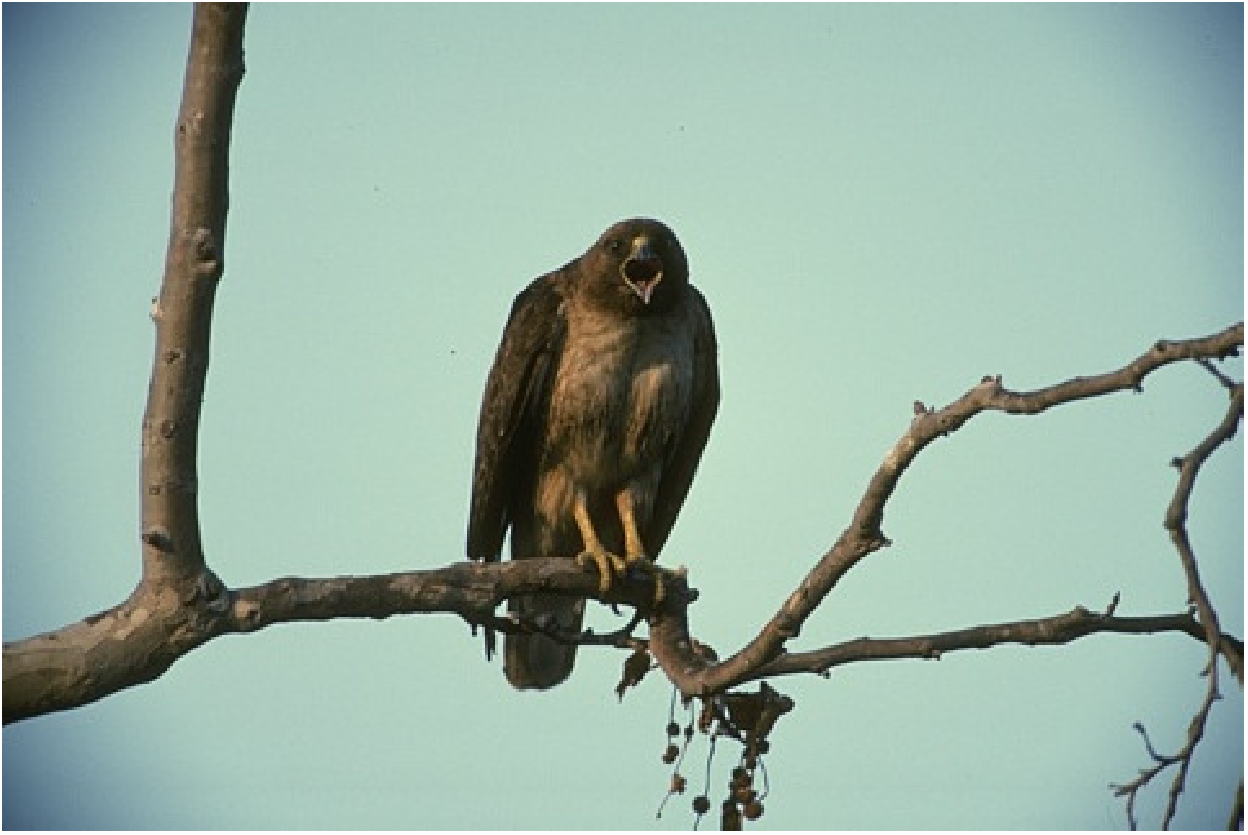
\includegraphics[width=0.47\linewidth]{teaser_img.pdf}\label{fig:teaser:input}}
\subfloat[Binary MAT]{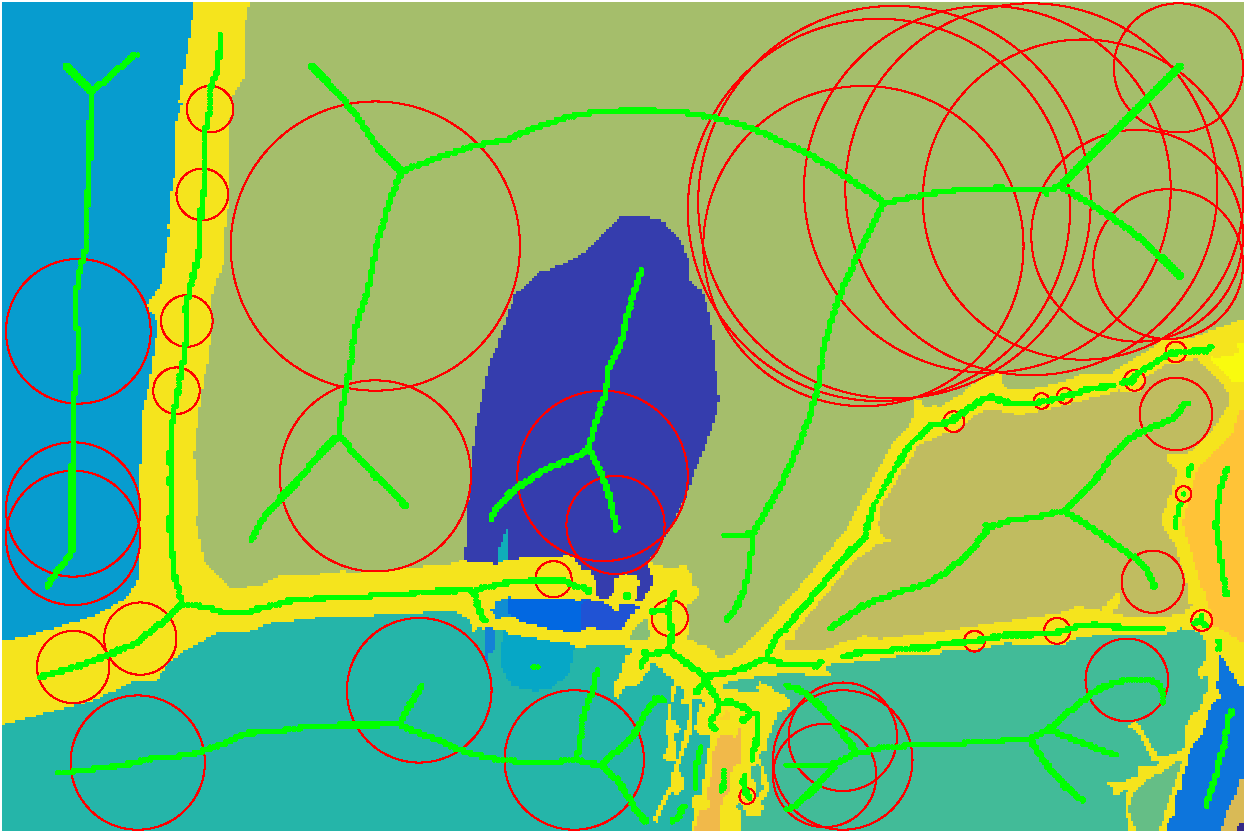
\includegraphics[width=0.47\linewidth]{teaser_mat.pdf}\label{fig:teaser:mat}} \\
\subfloat[Appearance-MAT]{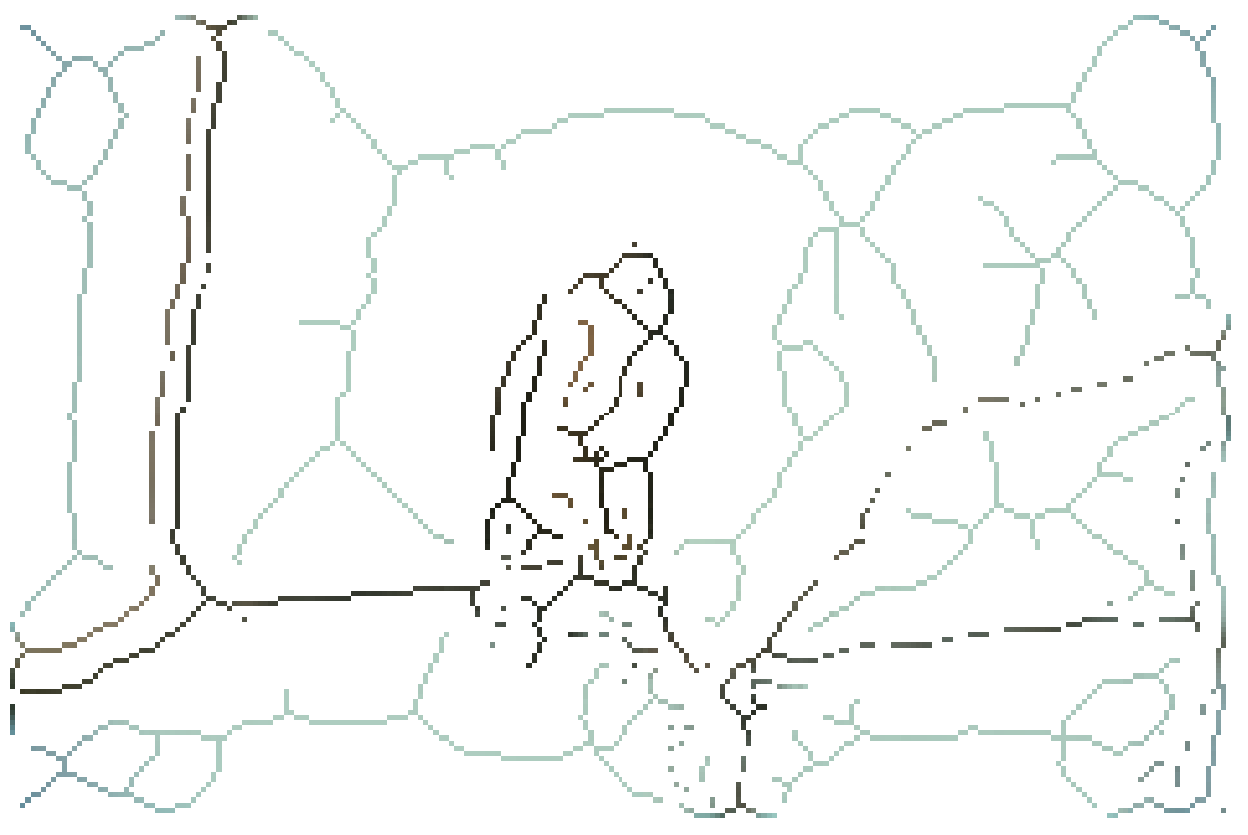
\includegraphics[width=0.47\linewidth]{teaser_amat.pdf}\label{fig:teaser:amat}}
\subfloat[Reconstructed image]{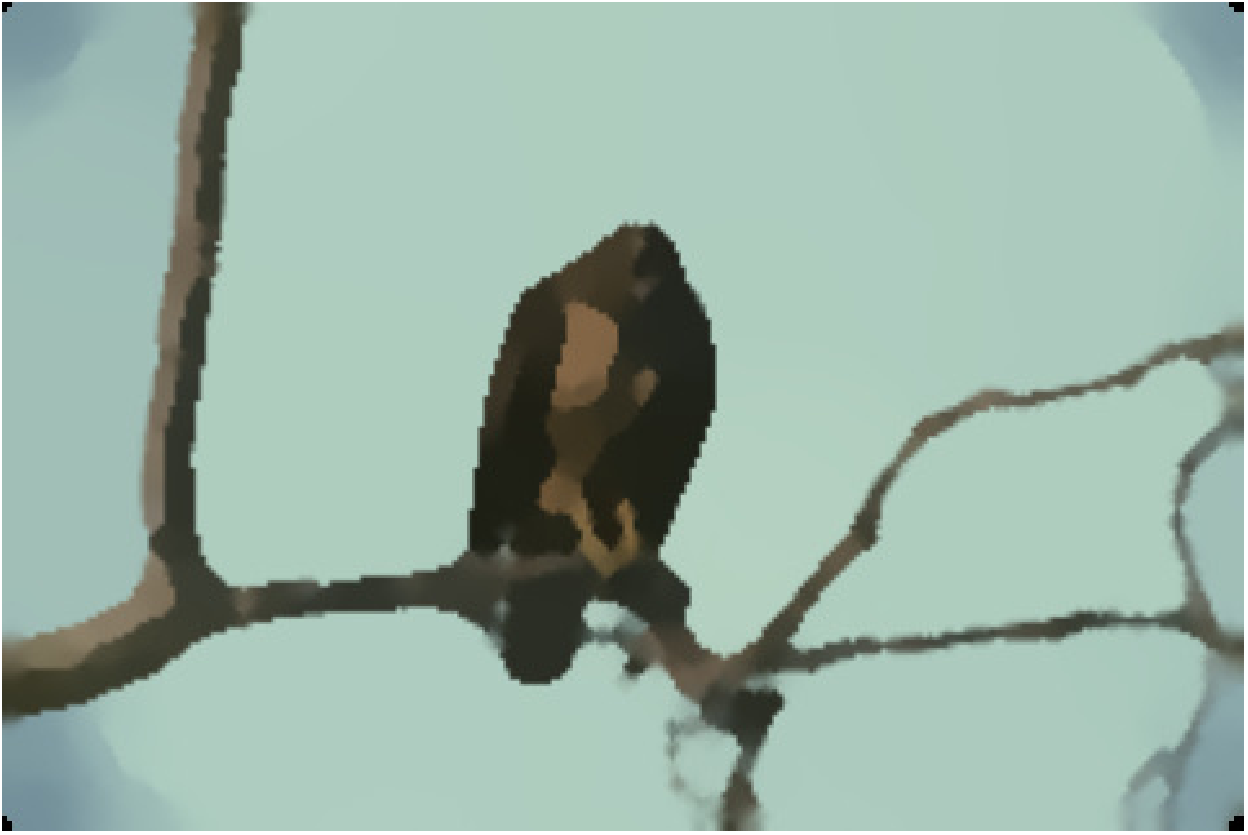
\includegraphics[width=0.47\linewidth]{teaser_recon.pdf}\label{fig:teaser:recon}}
\caption{\textbf{Top:} Input image (\ref{fig:teaser:input}) and segmentation (\ref{fig:teaser:mat}) from BSDS500,
using a different color for each ground-truth segment. 
Medial axes extracted from each segment using~\cite{telea2002augmented} (green) and a subset of medial disks (red) are overlaid. 
Using the medial disk radius information, we can reconstruct the input segments. 
\textbf{Bottom:} Similarly, the Appearance-MAT (\ref{fig:teaser:amat}) carries enough information to reconstruct the 
 \emph{input image} (\ref{fig:teaser:recon}) with just $\sim 5\%$ of the pixels 
 (we use white color for non-medial points in~\ref{fig:teaser:amat}).}
\label{fig:teaser}
\end{figure}

Symmetry is a ubiquitous property in the natural world, with a well-established role in human vision.
Humans instinctively recognize and use symmetry to analyze complex scenes, as it facilitates the encoding of shapes and
their discrimination and recall from memory~\cite{barlow1979versatility,royer1981detection,wagemans1998parallel}.
In the context of computer vision, \emph{local} symmetry is of particular interest, 
because of its robustness to viewpoint changes and its connection to salient structures, such as object parts.
This intuition is fundamental in many milestones in object representation theory, including generalized
cylinders~\cite{binford1971visual}, superquadrics~\cite{barr1981superquadrics}, 
geons~\cite{biederman1987recognition}, and shock graphs~\cite{siddiqi1999shock}.

Fundamental notions of local symmetry were introduced decades ago by Blum in the context 
of binary shapes with the \emph{medial axis transform (MAT)}~\cite{blum1967transformation,blum1973biological}.
The MAT is a powerful shape abstraction that has been successfully used in recognition, matching and retrieval. 
One of its most important strengths is that it provides a very compact representation that preserves the topological
properties of the input shape.
This makes the MAT very useful for reducing the computational complexity of various algorithms,
\eg for mesh editing~\cite{li2001decomposing,yoshizawa2003free} and shape manipulation~\cite{du2004medial},
and many researchers have tried to achieve a good balance
between MAT sparsity and reconstruction quality~\cite{tam2003shape,li2015q}.

Extending the notion of the MAT to natural images would correspondingly benefit applications that rely on
a sparse set of highly informative keypoints/landmarks, such as registration~\cite{zhou2016estimating}, 
retrieval~\cite{sivic2003video}, pose estimation and body tracking~\cite{shotton2013efficient},
and structure from motion~\cite{agarwal2011building}.
It would also assist segmentation, by enforcing region-based constraints through their medial point representatives
~\cite{teo2015detection}; and by providing a practical alternative to manual 
scribbles/seeds for interactive segmentation~\cite{boykov2001interactive,price2010geodesic,isack2016hedgehog,lin2016scribblesup}.

Unfortunately, the lack of a definition and an evaluation criterion 
that accommodate color and texture have prevented the widespread use of the MAT for tasks involving natural images.
Previous works have mostly attacked the sub-problem of \emph{medial point detection}~\cite{tsogkas2012learning,shen2016object},
which amounts to determining the \emph{locations} of points lying on medial axes 
but not the scale of the respective medial disk.
The type of axes considered is also constrained to make the problem more concrete:
\cite{tsogkas2012learning} only considers elongated structures, lying on both foreground objects and background; 
~\cite{shen2016object} instead focuses on \emph{object skeletons}, ignoring background structures.
These methods also lack a key characteristic of the MAT: medial point locations alone do not provide sufficient
information to reconstruct the input.

In this paper we introduce the first ``complete'' MAT for natural images, dubbed \emph{Appearance-MAT (AMAT)}.
First, we provide a new definition in the context of natural images by framing MAT 
as a weighted geometric set cover (WGSC) problem.
Our definition is centered around the MAT invertibility property and elicits 
a straightforward criterion for quality assessment, in terms of the reconstruction of the input image.
Second, our algorithm associates each medial point with \emph{scale} as well as local \emph{appearance} information
that can be used to reconstruct the input.
Thus, the AMAT encompasses all the fundamental features of its  binary counterpart. 
Third, we describe a simple bottom-up grouping scheme that exploits the additional scale and appearance information to connect
points into medial \emph{branches}.
These branches correspond to meaningful image regions, and extracting them can support image segmentation,
and object proposal generation, while offering a shape decomposition of the underlying structure as well. 

Being bottom-up in nature, our method does not assume object-level knowledge.
It computes medial axes of both foreground and background structures, 
yielding a compact representation that only uses $\sim 10\%$ of the image pixels.
Yet, this sparse set of points carries most of the signal present in the full image;
%enough information to reconstruct the input, and
%and can replace it in algorithms for high-level tasks, 
%(scene classification, image retrieval), significantly reducing their running time.
this differs from other sparse image descriptions, \eg edge maps, which strip the input of all appearance information.

We perform experiments in medial point detection on a new dataset of medial axes, the 
\emph{Berkeley-Medial AXes (BMAX500)}, which is built on the popular BSDS500 dataset, showing \sota\ performance.
We also measure the quality of reconstructions  obtained by inverting the AMAT of images from the same dataset, 
using  a variety of standard image quality metrics.
We compare with two reconstruction baselines: one built on the medial point detection algorithm from~\cite{tsogkas2012learning}
and one built from the ground-truth segmentations in BSDS500.
Our method significantly outperforms the baselines in terms of reconstruction quality, while attaining a $11\times$ compression ratio.

The outline of the paper is as follows: we start by reviewing related work on medial axis extraction for binary shapes
and natural images in~\refsec{sec:related}.
In~\refsec{sec:method} we describe our approach.
%we define the problem, introduce notation, and highlight the connection to the WGSC problem.
%We also discuss the schemes for bottom-up grouping of the medial points into branches and the AMAT simplification.
\refsec{sec:implementation} includes implementation details and in~\refsec{sec:experiments} we present our results.
Finally, in~\refsec{sec:discussion} we conclude and discuss ideas for future directions.


% ====================================================================================================================
\section{Related Work}\label{sec:related}
% ====================================================================================================================
\subsection{MAT for Binary Shapes}\label{sec:related:binary}
Blum introduced the concept of the medial axis transform, or skeleton, for 2D shapes
in his seminal works~\cite{blum1967transformation,blum1973biological}.
Since then, researchers have developed algorithms for reliable
and more efficient medial axis extraction, its extension to 3D shapes, and its application
to computer vision tasks.

Siddiqi~\etal define \emph{shocks} as the singularities of a curve evolution process acting on the boundaries of
a shape, and they organize them into a directed, acyclic shock graph~\cite{siddiqi1999shock}.
Shock graphs were successfully used in shape matching~\cite{siddiqi1999shock}, recognition~\cite{sebastian2001recognition},
and database indexing~\cite{sebastian2002shock}.
\emph{Bone graphs}~\cite{macrini2008skeletons} offer improved stability and a more intuitive representation of an object's parts, 
compared to skeletons and shock graphs, by identifying and analyzing ligature structures.
Visual part correspondences are also established and used to measure part and aggregated shape similarity in~\cite{latecki2000shape}.
The idea of object parts corresponding to endpoints of skeleton branches is further explored in~\cite{bai2008path}, where
\emph{geodesic} paths between skeleton endpoints are used to match the respective graphs.
More recently, Stolpner \etal deal with the problem of approximating a 3D solid via a union
of overlapping spheres~\cite{stolpner2012medial}.

The value of the MAT has been equally appreciated by the graphics community, where object shapes 
are routinely represented as point clouds or triangular meshes.
Giesen~\etal~\cite{giesen2009scale} introduced the \emph{scale axis transform}, a skeletal shape representation
that yields a hierarchy of successively simplified skeletons, which are obtained by multiplicative scaling of the
MAT's radii.
Li~\etal~\cite{li2015q} use quadratic error minimization to compute an accurate linear approximation of the MAT, called \emph{Q-MAT}.
They show experiments on medial axis simplification where they reduce the number of nodes of an initial medial mesh
by three orders of magnitude, while preserving good surface reconstruction.


\subsection{MAT for Natural Images}\label{sec:related:natural}
Compared to the binary setting, the number of works on medial axis detection for natural images is rather limited.
Levinstein \etal~\cite{levinshtein2009multiscale} detect \emph{symmetric parts} of objects
by learning to merge adjacent deformable maximally inscribed disks, modeled as superpixels.
Learned non-accidental part attachment relations are then used to combine proximal detected parts into coarse skeletal representations.
Lee \etal extend that work by introducing a deformable disk model that can capture curved and tapered parts, and also add
continuity constraints to the medial point grouping process~\cite{lee2013detecting}.
In other works medial point detection is posed as a classification problem where pixels are labeled
as ``medial'' or ``not-medial'', inspired by similar methods for boundary detection~\cite{martin2004learning}.
Tsogkas and Kokkinos use multiple instance learning (MIL) to deal with the unknown scale and orientation 
during training~\cite{tsogkas2012learning}, while Shen \etal adapt a CNN with 
side outputs~\cite{xie2015holistically} for \emph{object skeleton} extraction~\cite{shen2016object}.
All these approaches exploit appearance information by incorporating some sort of machine learning algorithm.

Our work can be regarded as lying at the intersection of previous work on binary and natural images.
From a technical standpoint, it shares more similarities with binary methods, for instance~\cite{stolpner2012medial},
which solves the set cover problem for volumes in the 3D space.
At the same time, it can be applied to real images, without assuming a figure-ground segmentation,
but it also demonstrates unique characteristics.
Our method does not involve learning, and is not constrained in detecting a particular subset of
medial axes as~\cite{tsogkas2012learning,shen2016object}.
It also complements existing methods by augmenting point locations with scale and appearance descriptions, which
are necessary for reconstructing the input.


% ====================================================================================================================
\section{Method}\label{sec:method}
% ===================================================================================================================

\begin{figure*}[t]
\centering
\def\imgw{0.245}
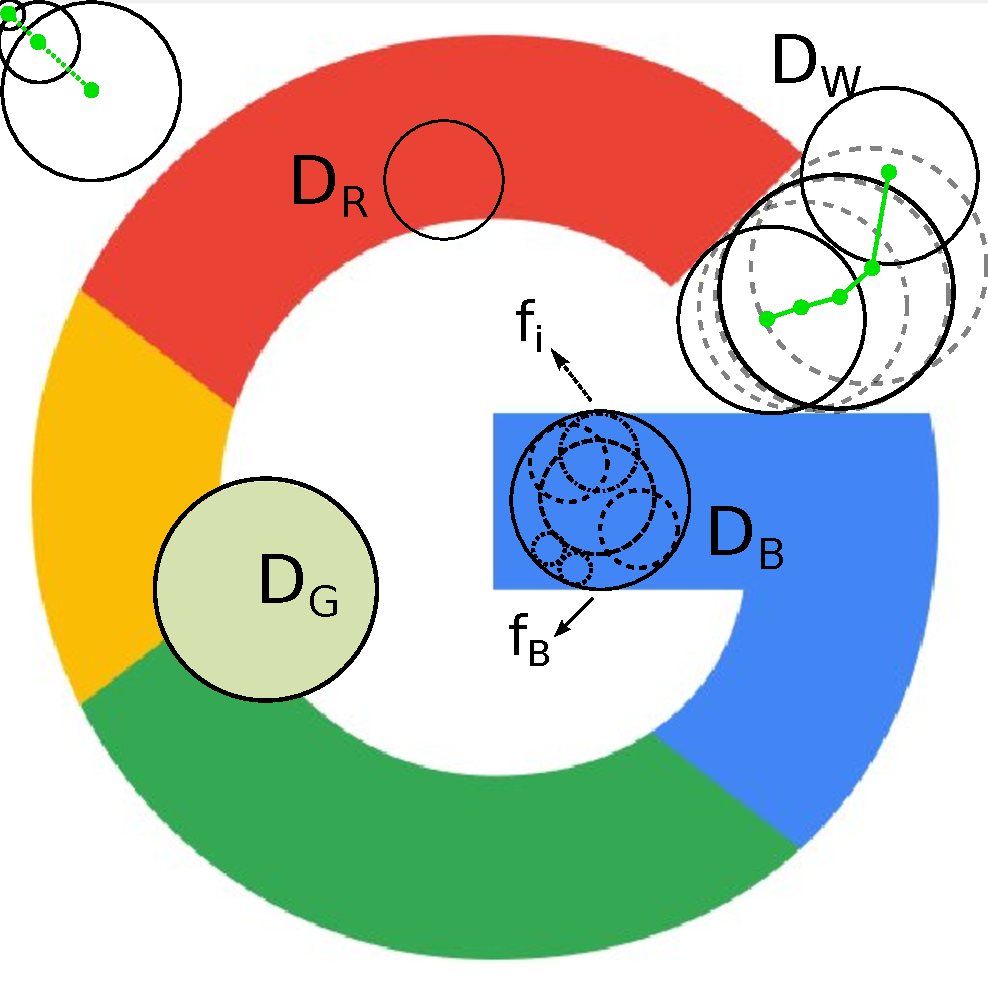
\includegraphics[width=\imgw\linewidth]{google_disks.pdf}
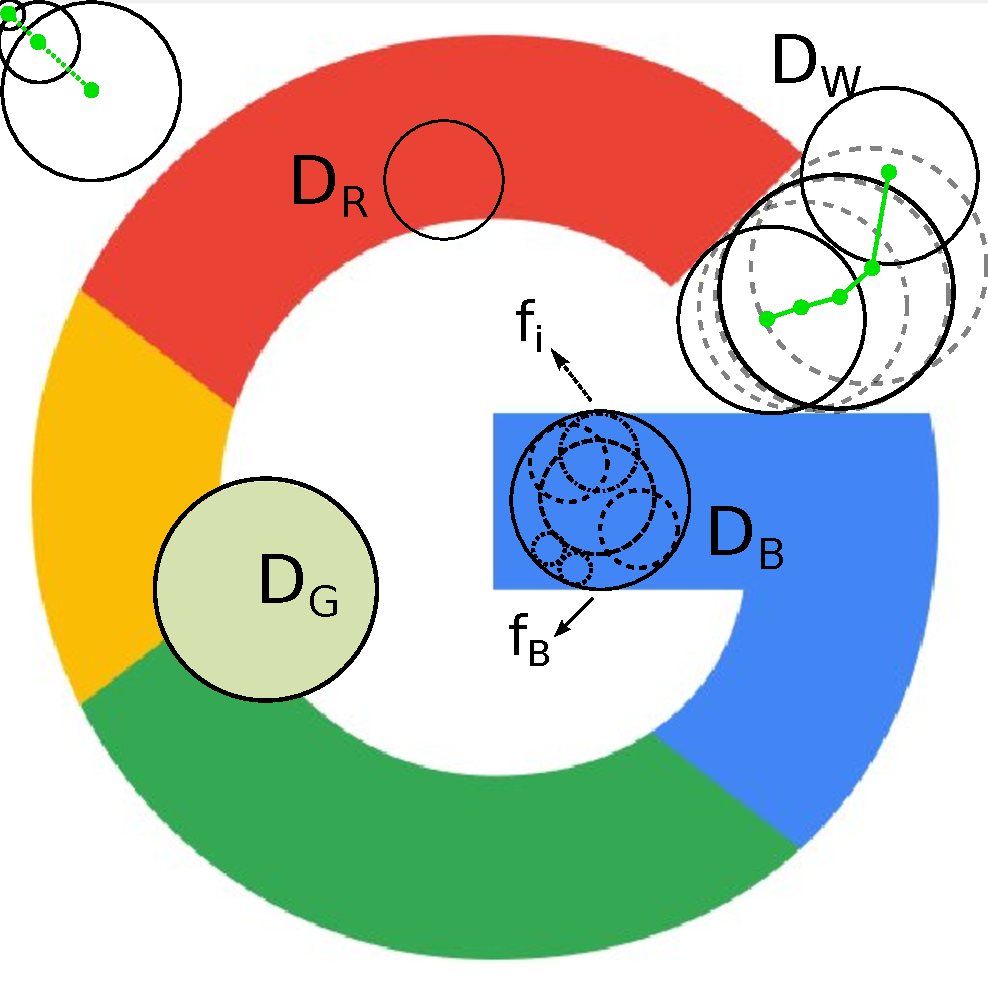
\includegraphics[width=\imgw\linewidth]{google_disks.pdf}
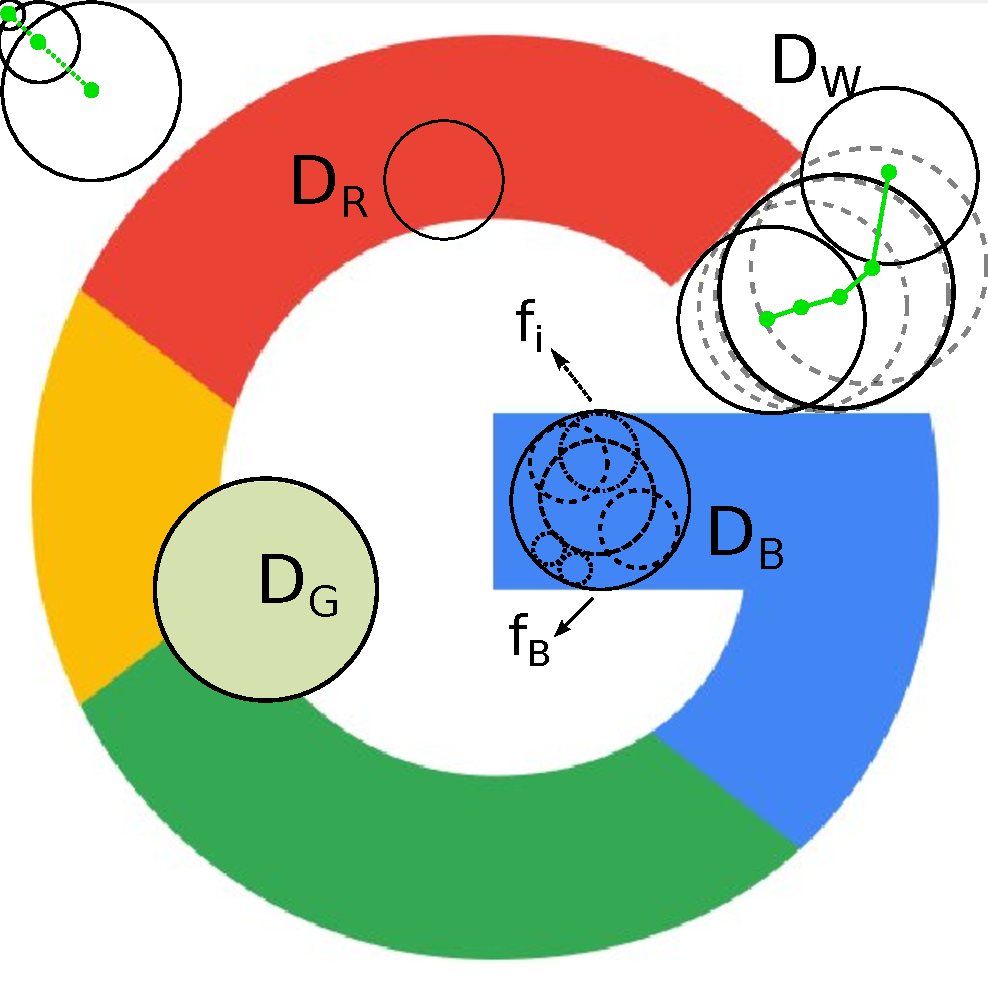
\includegraphics[width=\imgw\linewidth]{google_disks.pdf}
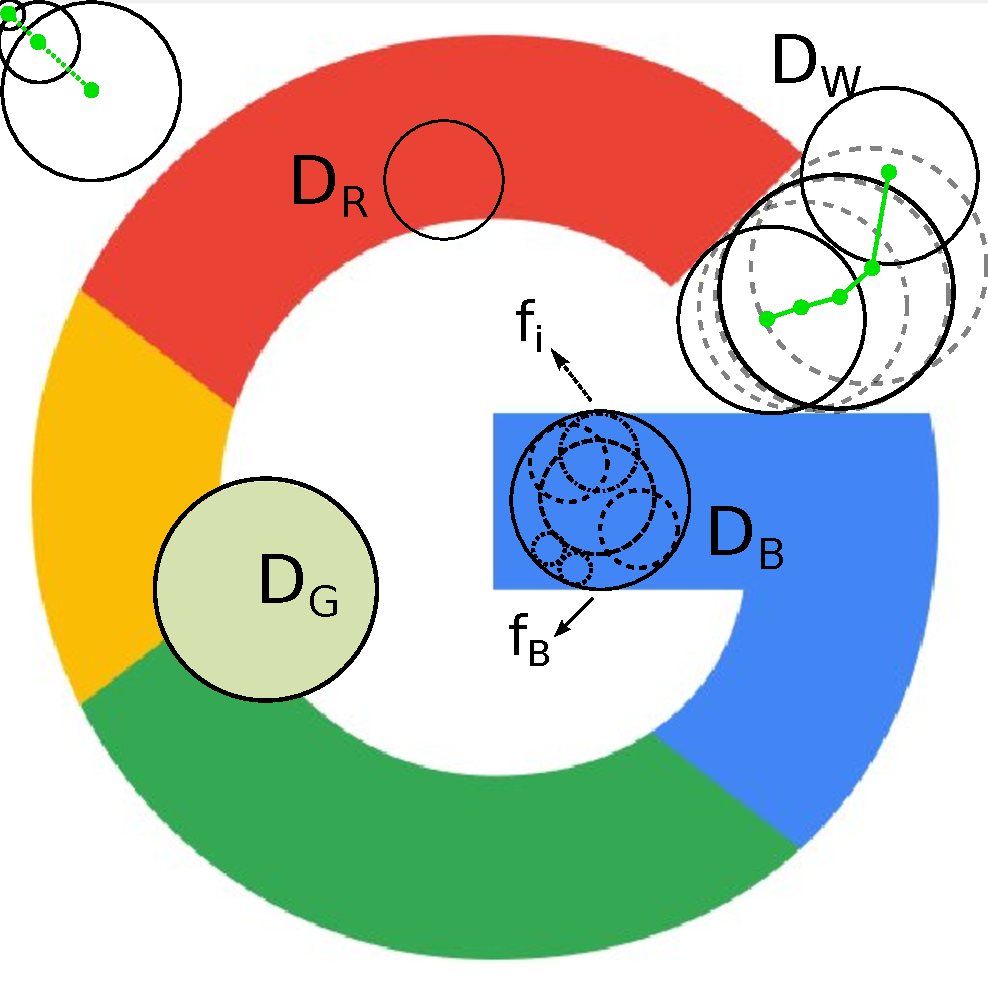
\includegraphics[width=\imgw\linewidth]{google_disks.pdf}
\caption{$\mathbf{D_W:}$ Composing an image using overlapping disks; disk centers form the medial axis (green points).
$\mathbf{D_G}$ lies at the intersection of three regions, so its encoding cannot accurately reconstruct the local image patch.
$\mathbf{D_R}$ incurs a small MSE, even though it does not respect region boundaries.
Comparing a disk's encoding $\f{B}$ to the encodings $\f{i}$ of \emph{all} contained disks provides a more robust
error metric.}
\label{fig:google}
\end{figure*}

\subsection{Problem Definition}\label{sec:method:definition}
Consider a 2D binary shape, $O$, in the image plane, and its boundary $\Theta_O$.
The \emph{medial axis} of $O$ is the set of points $\p{}$ that
%lie midway between two sections of its boundary. The points $\p{}$ 
are centers of the maximally inscribed (medial) disks, bitangent to $\Theta_O$
in the interior of the shape. The disk radius $r(\p{})$, called the \emph{medial radius}, 
is the distance between $\p{}$ and the points where the disk touches $\Theta_O$.
The process of mapping $O$ to the set of pairs $(\p{},r(\p{})) \in \mathbb{R}^2 \times \mathbb{R}$
is called the \emph{medial axis transform} (MAT).
Given these pairs, we can reconstruct the object as a union of overlapping disks that sweep-out 
its interior by ``expanding'' a value of one (1) inside the area covered by each  medial disk.

We argue that a MAT for real images should satisfy a similar principle: given the MAT of an image, 
we should be able to ``invert'' it, reconstructing \emph{the image} itself.
There are several reasons why extending this idea to real images is a challenging task. 
Natural images contain complex scenes and are cluttered with various objects, instead of a single foreground shape.
Moreover, whereas binary images are composed of uniform areas of zeros (0) and ones (1), 
real images obey complicated color and texture distributions.
Nevertheless, we can exploit image redundancies and assume that an image is composed of many small regions of 
relatively uniform appearance.
This is a concept on which most superpixel algorithms rely on for breaking up an image 
into non-overlapping patches, while respecting perceptually meaningful region 
boundaries~\cite{shi2000normalized,levinshtein2009turbopixels,achanta2012slic}. 
\paragraph{Notation:} Before proceeding with our formulation, we list the notation used throughout the paper.
We use capital italics for single elements and capital calligraphic letters to denote sets. A disk of radius $r$,
centered at point $\p{}$ is denoted as $D(\p{},r)=D_{\p{},r}$. 
For brevity, we often refer to such a disk as a $r$-disk or $(\p{},r)$-disk.
We will also occasionally use $r(\p{}) = r_{\p{}}$ to refer to the radius/scale $r$, associated with point $\p{}$.
$\set{D}$ is a collection of such disks of varying centers and radii, $\set{D}=\{ D_{\p{i},r_{\p{i}}} \},\, i\in\mathbb{N}$.
The intersection of a $(\p{},r)$-disk with an image $I$ is a disk-shaped region of the image, and is denoted by 
$I \cap D_{\p{},r}=D_{\p{},r}^I \subset I$. Finally, we use $\circ$ to denote function composition.

\paragraph{Formulation:} Consider an RGB image $I\subset\R^3$, and a disk-shaped region $D_{\p{},r}^I \subset I$.
Let $f:\R^3 \rightarrow \R^K$ be a function that maps $D_{\p{},r}^I$ to a vector  $\f{\p{},r}=f\circ D_{\p{},r}^I$; 
we call $\f{\p{},r}$ the \emph{encoding} of $D_{\p{},r}^I$. 
Now let $g:\R^K \rightarrow \R^3$ be a function that maps $\f{\p{},r}$ back to a disk patch 
$\tilde{D}_{\p{},r}^I = \g{\p{},r} = g \circ \f{\p{},r}$. We call $g$ the \emph{decoding} function.
In the general case, $f$ and $g$ will be \emph{lossy} mappings, which means that the reconstruction error 
$e_{\p{},r} = \norm{ \tilde{D}_{\p{},r}^I - D_{\p{},r}^I}_2^2 \geq 0$. 
Using the above, we define the AMAT as the set of tuples 
$M:\{ ( \p{1},r_{\p{1}}, \f{\p{1},r_{\p{1}}} ), \ldots, ( \p{m},r_{\p{m}}, \f{\p{m},r_{\p{m}}} ) \}$, such that:
\begin{equation}
M = \argmin_{\p{},r}{\sum_{i=1}^m e_{\p{i},r_i}},\quad I=\bigcup_{i=1}^m D_{\p{i},r_i}^I 
\label{eq:minimization}
\end{equation}
\refeq{eq:minimization} does not impose constraints on the number of points $m$;
we discuss this later in the text.
\paragraph{Encoding and decoding functions:}
Our framework allows $f,g$ to take any form; 
for example, $f$ could be a histogram representation of color in $D_{\p{},r}^I$ and $g$ could return the mode of the distribution.
In this paper we opt for simplicity:
$f$ computes the mean of each color channel ``summarizing'' $D_{\p{},r}^I$, in a $3\times1$ vector $\f{\p{},r}$.
Conversely, $g$ constructs an approximation $\tilde{D}_{\p{},r}^I \approx D_{\p{},r}^I$ by replicating $\f{\p{},r}$ in the
respective disk-shaped area.
When the $(\p{},r)$-disk is fully enclosed in a uniform region the reconstruction error $e_{\p{},r}$
is low, whereas when the disk crosses a strong image boundary, the encoding $\f{\p{},r}$ cannot accurately represent
the underlying image region, resulting in a higher error. 
%Because we augment each point by adding local appearance information in the form of $\f{\p{},r}$, 
%we dub our approach \emph{Appearance}-MAT or \emph{AMAT}.

Note that the definition in~\refeq{eq:minimization} suggests conceptual similarities with superpixel representations.
Selecting the points $\{ (\p{i},r_i,\f{\p{i},r_i}) \},\,i=1,\ldots,m$ is equivalent to covering the input image
with $m$ disk-shaped superpixels. Minimizing the total reconstruction error implies that these ``superdisks'' do not
cross region boundaries, as this would incur a high reconstruction error, as shown in~\reffig{fig:google}.
However, there are two important differences:
First, in our case a canonical shape (disk) is used, whereas superpixels can have any form. 
Second, our disks are \emph{overlapping}, in contrast to standard, non-overlapping superpixels.

\subsection{AMAT as a Geometric Set Cover Problem}\label{sec:method:wgsc}
The geometric set cover is the extension of the well studied set cover problem, in a geometric space.
Here we only consider the case of a two-dimensional space and we particularly focus on the 
\emph{weighted} version of the problem, which is defined as follows:
Consider a universe of $N$ points $\set{X} \in \R^2$ and subsets
$\set{D} = \{D_1,D_2,\ldots,D_k\} \subseteq \set{X}$, called \emph{ranges}. 
A common choice for $D_i$ is intersections of $\set{X}$ with simple shape primitives, such as disks or rectangles.

Now assume that each set in $\set{D}$ is associated with a non-negative weight or \emph{cost} $c_i$.
Solving the WGSC problem amounts to finding a sub-collection $\bar{\set{D}} \subset \set{D}$ that covers the entire $\set{X}$
(all $N$ elements of $\set{X}$ are contained in at least one set in $\bar{\set{D}}$), while having the minimum
total cost $C$; the total cost is simply the sum of costs of individual elements in $\bar{\set{D}}$.
WGSC is a strongly NP-hard problem for which polynomial-time approximate solutions (PTAS) exist.
The interested reader can find more details on WGSC and related algorithms 
in~\cite{mustafa2015quasi,varadarajan2010weighted,har2012weighted,chan2012weighted}.

The AMAT formulation described in~\refsec{sec:method:definition} lends itself naturally to a 
WGSC interpretation.
The spatial support $X^I$ of an input image $I$, is the universe of $N$ points.
As $\set{D}$ we consider the set of $r$-disks with $r$ chosen from a finite set $\set{R}:\{r_1,r_2,\ldots,r_R\}$.
The $r$-disks can be placed at any position $\p{}=(x,y)\in X$ such that $D_{\p{},r}$ is fully contained in $X$.
We also assign a cost $c_{\p{i},r_j} = c_{ij}$ to each possible $(\p{i},r_j)$-disk, $i\in[1,N],\, j\in[1,R]$.
This cost is directly related to the reconstruction cost 
$e_{\p{i},r_j} = e_{ij}$, given the functions $f,g$.
Note that for brevity, we drop the subscripts $\p{i},r_j$ and simply use $ij$ to refer to a $(\p{i},r_j)$-disk.
We provide more details regarding computation of $e_{ij}$ in~\refsec{sec:implementation}.

As~\refeq{eq:minimization} suggests, the goal is to find a subset of disks that cover the entire image, while maintaining
a low total reconstruction cost. 
A trivial solution would be to select each pixel as a disk of radius $r=1$, in which case
$M:\{ (\p{1},r_{\p{1}},f_{\p{1},r_{\p{1}}}), \ldots, ( \p{N},r_{\p{N}},f_{\p{N},r_{\p{N}}} ) \}$,
and $\sum_{i=1}^N e_{\p{i},r_i} = 0$; each pixel can be perfectly represented by its mean value.
Such a solution is of no practical use. 
Staying true to the spirit of the MAT, we seek a solution that is \emph{sparse}
(low number of medial points $m$), while being able to adequately reconstruct the input image.
One possible way to do this would be to agree on a fixed ``budget'' of points, and look for the 
optimal solution given $m$.
However, choosing an acceptable $m$ can be a nuisance, as its value can vary significantly  from image to image.

In the original MAT sparsity is implicitly induced through the use of maximal disks,
touching the shape boundary at two points or more.
Extending the maximality principle to real images is not straightforward;
because color and texture boundaries are not robustly defined.
Relying on the output of an edge extraction algorithm is not an option either,
as it would make our method sensitive to errors from which it would be impossible to recover.

We choose to regularize the minimization criterion in~\refeq{eq:minimization} in an alternative way. 
We add a scale-dependent term $s_j = \frac{w_s}{r_j}$ to the costs $c_{ij}$, with $s_j$ 
being inversely proportional to the radius $r_j$.
This way we favor the selection of larger disks at each point, as long as $s_j$ is not ``too'' large
with respect to the error incurred by picking $D_{\p{},r_{j+1}}$ instead of $D_{\p{},r_j}$.
Selecting a high value for $w_s$ leads to a sparser solution with higher total reconstruction error,
whereas a low value for $w_s$ aims for a better reconstruction, by utilizing more, smaller disks
to cover $X^I$.
~\reffig{fig:smoothing} shows how varying $w_s$ removes fine details, reconstructing only the most important structures.

\paragraph{Greedy approximation algorithm:}
There are many polynomial-time-approximate-solution (PTAS) algorithms for the vanilla set cover problem
and its geometric variants.
Since this is the first attempt at applying a WGSC approach to compute the MAT of real images, we keep things simple
and use the greedy algorithm described in~\cite{vazirani2013approximation}, adapted for the weighted case.
The steps of our method are described in~\refalg{alg:greedy}
\begin{algorithm}[t]
\caption{AMAT greedy algorithm.}
\label{alg:greedy}
	\begin{algorithmic}[1]
	\Statex \textbf{Input:} $X^I=\{\p{1},\ldots,\p{N}\},\set{R}=\{r_1,\ldots,r_R\},f,g$
	\Statex \textbf{Output:} $M$
	\State Initialization: $M \leftarrow \emptyset,X^c \leftarrow \emptyset$ \Comment{$X^c:$ covered pixels}.
	\State Compute $f_{\p{},r},\, g_{\p{},r} = g \circ f_{\p{},r},\,\, \forall \p{} \in I, \forall r \in \set{R}$
	\While{$X^c \subset X^I$}
		\State $c_{\p{},r}^e = \frac{c_{\p{},r}}{|D_{\p{},r} \setminus X^c|}+\frac{w_s}{r},\,\, \forall \p{} \in X^I, \forall r \in \set{R}$
		\State $(\p{}^{*},r^{*}) \leftarrow \argmin_{\p{},r}{c_{\p{},r}^e}$		
		\State $M\leftarrow M\cup{(\p{}^{*},r^{*},f_{\p{}^{*},r^{*}})}$
		\State $X^c \leftarrow X^c \cup D_{\p{}^{*},r^{*}}$ 
	\EndWhile
	\end{algorithmic}
\end{algorithm}
We start by computing the costs $c_{ij}$ for all possible disks $D_{ij}$.
We define the \emph{effective cost} of $D_{ij}$ as $c_{ij}^e = \frac{c_{ij}}{A_{ij}} + s_j$ , where $A_{ij}$ is the number
of \emph{new} pixels covered by $D_{ij}$ (pixels that have not been covered by a previously selected disk).
Starting from an empty set $M$, we pick the disk with the lowest $c_{ij}^e$ and add it to the solution, 
removing the area $D_{ij}$ from the pixels that have to be covered.
This process is repeated until all image pixels have been covered by at least one disk.

\subsection{Grouping Medial Points Into Branches}\label{sec:method:grouping}
The scale and appearance associated with each medial point provide a rich
description that can be used to group points belonging to the same region into \emph{medial branches}.
The beneficial effects of grouping in low-level vision tasks have been
observed in previous works~\cite{felzenszwalb2006min,zhu2007untangling,kokkinos2010highly,qi2015making}.
In our case, grouping pixels into branches can help us refine the final medial axis, 
by aggregating consensus from neighboring points, and break the image into meaningful regions.

We group detected medial points using an agglomerative scheme that starts at fine scales and
progressively merges together nearby points at coarser scales.
Our grouping criterion relies on proximity in \emph{scale-space} and \emph{appearance}.
Intuitively, points that are very close have higher probability of belonging to the same branch.
We also expect that the scale of neighboring points on the same branch will change \emph{gradually},
so points that lie close to each another but have very different scales should probably not be grouped together.
Finally, two points should not be merged if their encoding appearance vectors are very dissimilar,
regardless of their proximity in scale-space. 
%as this indicates that they belong to different regions, 

We initialize branches as the connected components of the AMAT output.
Starting at a scale $r_j$, we consider one branch at a time, and examine all other
branches within a neighborhood of size $r_j \times r_j$ and a scale neighborhood $[r_{j-3},r_j]$.
If two branches coexist in this scale-space neighborhood and their average encodings 
(summed along the branch curve) are similar, they are merged.
The grouping algorithm terminates when all scales have been considered.

%\begin{algorithm}[t]
%\caption{Point grouping algorithm.}
%\label{alg:grouping}
%	\begin{algorithmic}[1]
%	\Statex \textbf{Input:} $\set{R}=\{ r_1,\ldots.r_R \}, \newline M=\{ (\p{i},r_{\p{i}},\mathbf{f}_{\p{i},r_{\p{i}}}) \}, \, i=\in[1,m]$.
%	\Statex \textbf{Output:} $B= \{ \mathbf{b}_1,\ldots,\mathbf{b}_k \} = \newline \{ (\p{l_{11}},\ldots,\p{l_{1i}}), \ldots, (\p{l_{k1}},\ldots,\p{l_{kj}}) \},\, l_{ij}\in[1,m]$.
%	\State Initialization: $B \leftarrow cc(M)$. \Comment{Connected components}
%	\ForAll{scales $r_i$}
%		\ForAll{branches $\mathbf{b}_j$}
%		\EndFor
%	\EndFor
%	\end{algorithmic}
%\end{algorithm}


\subsection{Medial Branch Simplification}\label{sec:method:simplification}
The output of our algorithm captures mostly region centerlines but there are still
imperfections in the form of noisy responses or ``lumps'', instead of thin contours.
Such imperfections are expected since the greedy algorithm provides only an approximate solution
to the minimization problem of~\refeq{eq:minimization}. 
In addition, because we use a discrete grid, the placement of disks 
in the image domain does not always result in their centers spanning a continuous curve, 
which leads to isolated medial points.

Grouping MAT points into branches makes it possible to process each branch individually, enabling
the correction of these errors post hoc.
We perform simple morphological operations (dilation and thinning) 
on the points of each branch to merge neighboring and isolated pixels together, while removing 
redundant responses. 
We also adjust the scales of the medial points after thinning, to ensure that the medial disks corresponding 
to the simplified structure span the same image area.
Because grouped branches correspond to relatively homogeneous regions, we expect that reconstruction
results after simplification will not change much.
Examples of simplified medial axes are illustrated in~\reffig{fig:experiments:detection:examples}.
With a negligible drop in reconstruction quality, we are able to achieve a dramatic reduction
in the number of medial points, and produce much cleaner medial axes.


% =============================================================================================
\section{Implementation Details}\label{sec:implementation}
% =============================================================================================
\subsection{Disk Cost Computation}\label{sec:implementation:diskcost}
The greedy algorithm described in~\refsec{sec:method:wgsc} requires assigning a cost to all possible disks $D_{ij}$.
Choosing an appropriate type of cost function is crucial towards obtaining a final AMAT that both 
yields a sparse solution, and faithfully reproduces the input image.
Since our objective is high reconstruction quality, $c_{ij}$ should be directly proportional
to the reconstruction error of the local image patch.
Using a criterion such as MSE is not effective;~\reffig{fig:google} shows that naively selecting a disk with 
a low MSE score does not guarantee that it respects image boundaries.
Instead, we would rather select disks whose encodings are representative of \emph{all} disks that are fully enclosed
in their area. 

First, we convert the RGB input image to the CIELAB color space which is more suitable for measuring perceptual distances,
and perform all our computations in that space.
We define the cost for a disk $D_{ij}$ as follows:
\begin{equation}
c_{ij} = \sum_k \sum_l \norm{\mathbf{f}_{ij} - \mathbf{f}_{kl} }^2 \quad \forall k,l: D_{kl} \subset D_{ij}
\label{eq:diskcost}
\end{equation}
Intuitively, a low cost $c_{ij}$ implies that the encoding $\mathbf{f}_{ij}$ is representative of \emph{all}
disks that are fully contained in $D_{ij}$, hence $D_{ij}$ is not crossing any region boundaries.

Computing $c_{ij}$ can be very demanding as it requires computing encoding differences for all 
disks in $D_{ij}$; if $r_j$ is large, this number can grow very quickly.
We discuss how we can significantly reduce computation time in the supplemental material.

%We can significantly reduce computation time by i) using convolutions to compute the sums in~\refeq{eq:diskcost};
%and ii) minimizing redundant computations by using cumulative sums over \emph{circular} areas instead of disks.
%An alternative way to speedup performance is using rectangular or square shapes as the
%shape elements we use to cover the image domain.
%Using square filters would allow us to compute sums within regions with a fixed number of operations per position on an integral
%image~\cite{viola2001rapid,arbelaez2011contour}, reducing complexity by an order of magnitude.
%We leave this as a future extension and include further details of our current implementation in the supplemental material.

\subsection{Dealing With Texture}\label{sec:implementation:texture}
The main motivation behind the choice of simple functions $f,g$,
such as the ones described in~\refsec{sec:method:definition}, was simplicity and  computational efficiency.
Such functions also allow us to inject certain desired characteristics into the regions depicted by medial points in the AMAT solution, 
including, for example, appearance uniformity and alignment with boundaries.
However, natural images often contain high-frequency textures or noise, which can lead to the accumulation of large errors 
in~\refeq{eq:diskcost}, and promote the selection of disks that do not correspond to perceptually coherent regions. 
Simple processing techniques (\eg Gaussian filtering) can reduce noise but they also degrade image boundaries and
blend together neighboring regions.

To alleviate this problem, we ``simplify'' the input image before extracting the AMAT, using a method that smooths high frequency
regions, while preserving important edges~\cite{xu2011image}.
In practice, this preprocessing produces an image that is  perceptually very similar to the original, 
but without high-frequency textures that can cause the greedy algorithm to fail by placing disks at undesired locations.

\subsection{Inverting the AMAT}\label{sec:implementation:inverting}
Generating the reconstruction of a single disk-shaped region, $\tilde{D}_{\p{},r}^I$, is trivially achieved by
replicating $\f{\p{},r}$.
However, since medial disks are overlapping, most pixels in the image domain will be covered by multiple disks,
with different encodings.
We resolve this ambiguity in a simple way: while extracting the AMAT of an image, we keep track of the
number of disks each pixel is covered by; this quantity is called the \emph{depth} in the context of the set cover problem.
We then use the average $\f{}$ of all disks covering a point $\p{i}$ with depth $d_i$ as its reconstructed value:
\begin{equation}
\tilde{I}(\p{i}) = \frac{\sum_{\p{},r} \f{\p{},r}}{d_{\p{}}} \quad \forall \p{},r: \p{i}\in D_{\p{},r}
\label{eq:reconstruction}
\end{equation}

\begin{figure*}
\def\img_id{41004}
\def\imgw{0.245}
\subfloat[Input image]{\includegraphics[width=\imgw\textwidth]{\img_id_smoothed.jpg}}\hfill
\subfloat[$w_s=10^{-4}$]{\includegraphics[width=\imgw\textwidth]{{\img_id_recon0.0001}.jpg}}\hfill
\subfloat[$w_s=10^{-3}$]{\includegraphics[width=\imgw\textwidth]{{\img_id_recon0.001}.jpg}}\hfill
\subfloat[$w_s=10^{-2}$]{\includegraphics[width=\imgw\textwidth]{{\img_id_recon0.01}.jpg}}\hfill
\caption{Using a progressively larger scale-cost factor $w_s$ removes details keeping only coarse image structures.}
\label{fig:smoothing}
\end{figure*}

\subsection{Parameter Values}\label{sec:method:parameter}
For the smoothing algorithm we use the default values $\lambda=2\cdot10^{-4}$ and $\kappa=2$ that 
the authors suggest for natural images~\cite{xu2011image}.
Regarding the scale cost term described in~\refsec{sec:method:wgsc}, we found that $w_s=10^{-4}$ is a value that 
strikes a good balance between reconstruction quality and sparsity of the generated medial axis.
$\set{D}$ comprises disks at $40$ different scales in total, with radii $r\in[2,41]$.








% ====================================================================================================================
\section{Experiments}\label{sec:experiments}
% ====================================================================================================================
We evaluate the performance of our method on two tasks: 
i) localization of medial points in an image; and
ii) generating accurate reconstructions of images, given their AMAT.

\subsection{Medial Point Detection}\label{sec:experiments:detection}
We want to emphasize the difference between the problem we are addressing, and the objectives pursued in other works.
In~\cite{tsogkas2012learning} the authors focus on detecting local reflective symmetries of elongated structures,
and they build a dataset with annotations of segments in the BSDS300 that fit this description.
As a result, a large portion of the segments in BSDS is not used in performance evaluation.
In~\cite{shen2016object} the authors are explicitly interested in extracting \emph{object}
skeletons, completely ignoring background structures.
Although extracting object skeletons may be convenient for some tasks, it does not constitute a generalized
notion of MAT.

In our work we do not make such distinctions. 
The central idea behind the AMAT is to be able to reproduce the full input image,
so we view all parts of the image as equally important.
This is also the reason we choose BSDS500 as a basis for constructing medial axes annotations.
BSDS500 contains multiple segmentations for each image, offering higher probability of
capturing segments at varying scales, making it more relevant to the problem we are trying to solve
than datasets with object-level annotations.

Following a similar approach to the one used in~\cite{tsogkas2012learning}, 
we individually process all segments in a given segmentation, applying a skeletonization 
algorithm~\cite{telea2002augmented} on their binary masks to extract \emph{segment skeletons}.
The medial axis ground truth for the image is formed by taking the union of all the segment skeletons, and this
process is repeated for all available segmentations for each image (usually 5-7).

To conduct a fair comparison, we retrain the MIL-based algorithm from~\cite{tsogkas2012learning} on BMAX500.
We also tried to retrain the CNN model used in~\cite{shen2016object}, but the outputs we obtained were too noisy, 
and not of any practical use.
We hypothesize that the reason for that is the lack of consensus among the multiple ground truth maps
available for each image, which leads to convergence problems for the network; this has been previously
reported in~\cite{xie2015holistically}.
%Unlike~\cite{xie2015holistically}, in our case it is impossible to enforce ground truth consensus,
%because the position discrepancies for medial axes extracted from different annotations are very high.
We evaluate performance using the standard precision, recall and f-measure metrics, 
and show results in~\reffig{fig:experiments:detection:pr}.
Note that our algorithm does not output a skeleton probability map, so plotting
PR-curves by varying a score threshold is not applicable in our case.
For all methods, detections within a distance of $1\%$ of the image diagonal from a ground-truth positive 
are considered as true positives.
We show qualitative results of the medial axes and the grouped branches in~\reffig{fig:experiments:detection:examples}.

\begin{figure}
\centering
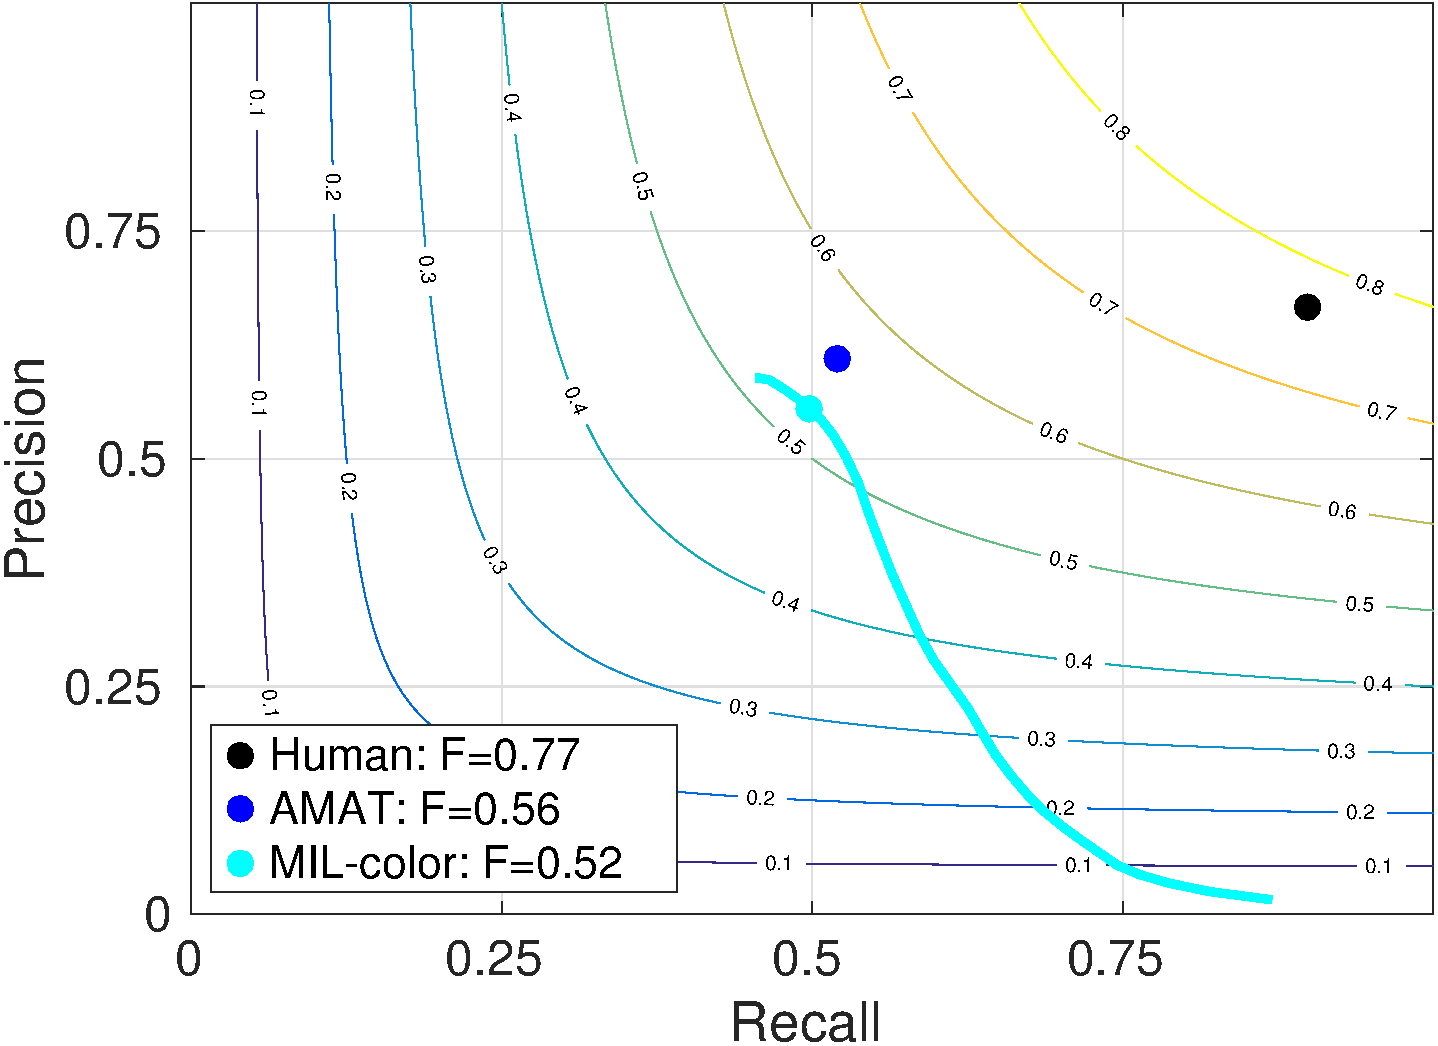
\includegraphics[width=0.9\linewidth]{pr.pdf}
\caption{Medial point detection in BMAX500 val set.}
\label{fig:experiments:detection:pr}
\end{figure}

\begin{figure*}[t]
\centering
\def\imgw{0.24}
\def\img_id{3096}
\includegraphics[width=\imgw \textwidth]{\img_id_resized.jpg}
%\includegraphics[width=\imgw \textwidth]{\img_id_smoothed_resized.jpg}
\includegraphics[width=\imgw \textwidth]{\img_id_axes_simplified.pdf}
\includegraphics[width=\imgw \textwidth]{\img_id_branches_simplified.pdf}
\includegraphics[width=\imgw \textwidth]{\img_id_gt_skel.pdf}

\def\img_id{253055}
\includegraphics[width=\imgw \textwidth]{\img_id_resized.jpg}
%\includegraphics[width=\imgw \textwidth]{\img_id_smoothed_resized.jpg}
\includegraphics[width=\imgw \textwidth]{\img_id_axes_simplified.pdf}
\includegraphics[width=\imgw \textwidth]{\img_id_branches_simplified.pdf}
\includegraphics[width=\imgw \textwidth]{\img_id_gt_skel.pdf}

%\def\img_id{85048}
%\includegraphics[width=\imgw \textwidth]{\img_id_resized.jpg}
%%\includegraphics[width=\imgw \textwidth]{\img_id_smoothed_resized.jpg}
%\includegraphics[width=\imgw \textwidth]{\img_id_axes_simplified.pdf}
%\includegraphics[width=\imgw \textwidth]{\img_id_branches_simplified.pdf}
%\includegraphics[width=\imgw \textwidth]{\img_id_gt_skel.pdf}

\def\img_id{295087}
\includegraphics[width=\imgw \textwidth]{\img_id_resized.jpg}
%\includegraphics[width=\imgw \textwidth]{\img_id_smoothed_resized.jpg}
\includegraphics[width=\imgw \textwidth]{\img_id_axes_simplified.pdf}
\includegraphics[width=\imgw \textwidth]{\img_id_branches_simplified.pdf}
\includegraphics[width=\imgw \textwidth]{\img_id_gt_skel.pdf}
\caption{\textbf{Medial axes}. From left to right: Input image, AMAT medial axes, medial branches (color-coded), ground-truth skeletons.
Axis color indicates the appearance in the respective medial region, and black is used for non-medial points. 
View in color and magnified.}
\label{fig:experiments:detection:examples}
\end{figure*}


\subsection{Image Reconstruction}\label{sec:experiments:reconstruction}
We now assess the quality of reconstructions we obtain by inverting the computed AMAT
of images from the BSDS500 dataset.
We compare with a baseline reconstruction algorithm based on the MIL approach 
of~\cite{tsogkas2012learning} (after retraining on BMAX500).
Their method produces a map of medial point strength at 13 scales and 8 orientations, for each pixel.
A single confidence value for each point is derived through a noisy-or operation,
which does away with scale and orientation information.
As a surrogate, in our experiments we associate each point with the scale/orientation combination
that has the highest medial point probability.

The scheme we use to create a crude reconstruction using the MIL-based approach is the following:
We start by sorting the medial point scores in decreasing order and we pick the one with the highest score.
The points under the rectangular region at the respective scale and orientation are then marked as covered,
and the process is repeated until the whole image has been reconstructed.
Point encodings are, similarly to our own method, the mean RGB values within the rectangular area, 
and local reconstructions are computed by averaging overlapping encodings.

We also compare with a second baseline, obtained by considering ground-truth segments in BSDS500
and representing them by their mean RGB values.
We show that an ``optimal'' sparse representation of the image, in the form of its human-annotated
boundaries and the encodings of the enclosed regions, results in much poorer reconstruction
quality compared to our approach.
We consider three standard evaluation metrics for image similarity: MSE, PSNR, and SSIM.
%We also examine an additional similarity criterion that has gained popularity recently, 
%in the context of convolutional neural networks.
%Specifically, we measure how close the reconstructed image is to the original,
%``in the eyes'' of a CNN, by computing the $L_2$ norms of feature maps at various layers. \stavros{say which layers}
Results are reported in~\reftab{tab:experiments:reconstruction} and visual examples are shown
in~\reffig{fig:experiments:reconstruction}.


\begin{table}
\centering
\begin{tabular}{|c|c|c|c|c|}
\hline
Metric	&	MSE		&	PSNR (dB)	&	SSIM	&	Compression 	\\
\hline
MIL~\cite{tsogkas2012learning}	&	0.0258	& 	16.6 	& 	0.53	&	$20\times$	\\
\hline
GT seg &	0.0220	& 	17.28 	& 	0.57	&	$15\times$\\
\hline
AMAT	&	\textbf{0.0058}	&	\textbf{22.74}	&	\textbf{0.74}	&	$11\times$	\\
\hline
\end{tabular}
\caption{Image reconstruction quality in BSDS500 val set.}
\label{tab:experiments:reconstruction}
\end{table}

\begin{figure*}[t]
\centering
\def\imgw{0.24}
%\def\img_id{3096}
%\includegraphics[width=\imgw \textwidth]{\img_id_resized.jpg}
%\includegraphics[width=\imgw \textwidth]{\img_id_rec_mil.png}
%\includegraphics[width=\imgw \textwidth]{\img_id_rec_gtseg.png}
%\includegraphics[width=\imgw \textwidth]{\img_id_rec_amat.png}

\def\img_id{145086}
\includegraphics[width=\imgw \textwidth]{\img_id_resized.jpg}
\includegraphics[width=\imgw \textwidth]{\img_id_rec_mil.png}
\includegraphics[width=\imgw \textwidth]{\img_id_rec_gtseg.png}
\includegraphics[width=\imgw \textwidth]{\img_id_rec_amat.png}

\def\img_id{85048}
\includegraphics[width=\imgw \textwidth]{\img_id_resized.jpg}
\includegraphics[width=\imgw \textwidth]{\img_id_rec_mil.png}
\includegraphics[width=\imgw \textwidth]{\img_id_rec_gtseg.png}
\includegraphics[width=\imgw \textwidth]{\img_id_rec_amat.png}

\def\img_id{42049}
\includegraphics[width=\imgw \textwidth]{\img_id_resized.jpg}
\includegraphics[width=\imgw \textwidth]{\img_id_rec_mil.png}
\includegraphics[width=\imgw \textwidth]{\img_id_rec_gtseg.png}
\includegraphics[width=\imgw \textwidth]{\img_id_rec_amat.png}

\caption{\textbf{Image reconstruction}. From left to right: Input image, MIL~\cite{tsogkas2012learning}, ground-truth segmentation, AMAT.}
\label{fig:experiments:reconstruction}
\end{figure*}



% ====================================================================================================================
\section{Discussion}\label{sec:discussion}
% ====================================================================================================================
We have proposed the first definition for the medial axis transform in natural images and described and algorithm for
computing it and evaluating its quality.
Our approach, called Appearance-MAT, or simply AMAT, bridges the gap between MAT methods for binary shapes and 
medial axis/local symmetry detection methods for real images.
We demonstrate \sota\ performance in medial point detection and show that we can produce a high-quality 
reconstruction of the input image using as few as $10\%$ of its pixels. 
A limitation of our framework is that it cannot deal with high frequency textures.
Using more powerful encoding/decoding functions $f,g$ could offer a solution to this problem.
Furthermore, the output of our algorithm offers a good starting set of salient regions, represented by 
their medial branches, which can be further merged to form object proposals.
We intend to explore these research directions in future work.


{\small
\bibliographystyle{ieee}
\bibliography{iccv2017.bib}
}

\end{document}
